\documentclass{article} 
\usepackage{nips12submit_e,times}
\usepackage{textcomp}
\usepackage{graphicx}
\pagestyle{empty}
\nipsfinalcopy

\title{Zero-Shot Learning for Human Action Recognition}
\author{Nicole Rafidi \\
  \texttt{nrafidi@cs.cmu.edu}
  \And
  Yuzuko Nakamura \\
  \texttt{yuzi@cs.cmu.edu}
  \And
  Danny Zhu \\
  \texttt{dannyz@cs.cmu.edu}
}

\begin{document}
\maketitle
\begin{abstract}
We demonstrate the performance of zero-shot learning (ZSL) for the task of human action recognition. Instead of training a classifier to map from low-level video-extracted features directly to action labels, we instead train $k$ regressors to map the videos to an intermediate semantic feature space.  Each action label is represented as a point in this feature space, and classification is then done by choosing the canonical action point that is closest to the query point.  This allows us to classify actions for which we have never seen video examples, a method of generalization that is important for improving the feasibility of human action recognition. Success of this method is evaluated as leave-two-out cross-validation (LTOCV) performance, and semantic feature comparison is shown using percent of variance explained (POVE).
\end{abstract}
\section{Introduction}
Zero-shot learning (ZSL) enables one to classify input into classes not yet seen in the training data. It does so by making use of a semantic knowledge base as an intermediate step between the features and classes \cite{Palatucci09}. The main objective of this project is to see whether zero-shot learning yields good performance in human action recognition. Human action recognition is a domain in which there are many possible class labels (actions), making it intractable to provide examples of each action in a training set \cite{Poppe10}. This makes it a good candidate for improvement by zero-shot learning.

\section{Related Work}

\section{Methods}

\subsection{Two-Stage Learning}
To test the efficacy of ZSL on this problem, we established two steps of classification on the videos in the data sets. First, we found a low-dimensional set of core features that can be used to distinguish the labels (running, walking, etc).  We designed the feature set based on our knowledge of human actions. A potentially better way to have selected this set would have been to mine text corpus statistics or to use psycholinguistic surveys. However, this is a proof of concept paper, so any reasonable feature set would be sufficient. 

Each action was described by a 12-dimensional vector. The features are represented as discrete values corresponding to some canonical aspect of an action (e.g. `Is there horizontal displacement?'). See section \ref{sf} for a list of the semantic features and their corresponding actions.

In the preprocessing stage, we extract low-level features from the videos using the interest points algorithm. Briefly, the interest points algorithm is a simple 3-dimensional generalization of Harris points. The points are selected as the local maxima of a particular function on the video which selects for large local variation in all directions \cite{Laptev05}.

An optical flow histogram (OFH) descriptor is then computed for each interest point. The x and y flow values in a neighborhood of a point are separately binned and the counts normalized. The two histograms are then concatenated to form the descriptor for each point. A single descriptor is made for a whole video with a bag-of-features model. All of the OFH descriptors from all training videos are taken together and clustered by k-means. Any video then is represented by the normalized histogram of the clusters to which its OFH descriptors belong \cite{Laptev04}.

These low-level features are used as input to the first stage of the classification process, in which 12 linear regressors are trained to map from the video features to the semantic features (one regressor per feature).  In the second stage, each action is represented by a point in this 12-dimensional feature space. To classify a video, the corresponding point is found. The action point which is the minimum distance away is the label selected. See figure \ref{2stage} for a summary.

A note on the measurement of distance: there are several ways to measure distance in multidimensional space. To be comprehensive, we used three measures of distance: Euclidean, Manhattan, and Cosine distance. To make a classification we select the action point that minimizes the sum of these three distance measures to the query point.
\begin{figure}[h]
\centering
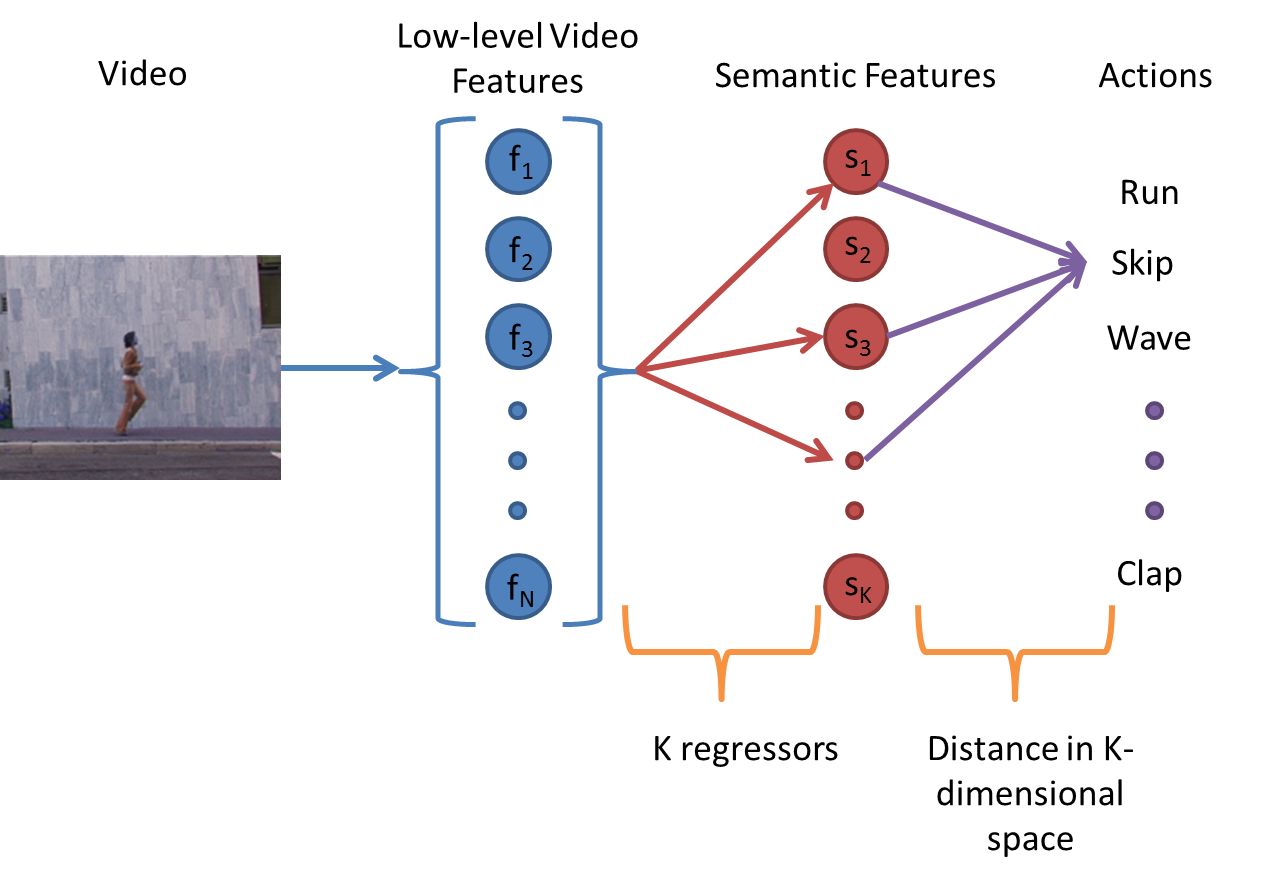
\includegraphics[width=.4\linewidth]{2stagelearning.png}
\caption{A summary of the two-stage learning process.}
\label{2stage}
\end{figure}
\subsection{Leave-Two-Out Cross-Validation}
To test the effectiveness of this two-step method over direct video-to-label mappings, we can perform leave-two-out cross-validation, and demonstrate the ZSL classifier’s ability to distinguish between two previously unseen class labels based on their video data, a task that direct mappings are unable to perform.

First, the 12 regressors are trained on all but two of the actions.  then, a video of a previously unseen action is presented. This produces a query point in semantic space.  The distance between the query point and the actual held-out action points is measured, and the point is classified. See figure \ref{ltocv} for a summary.

\begin{figure}[h]
\centering
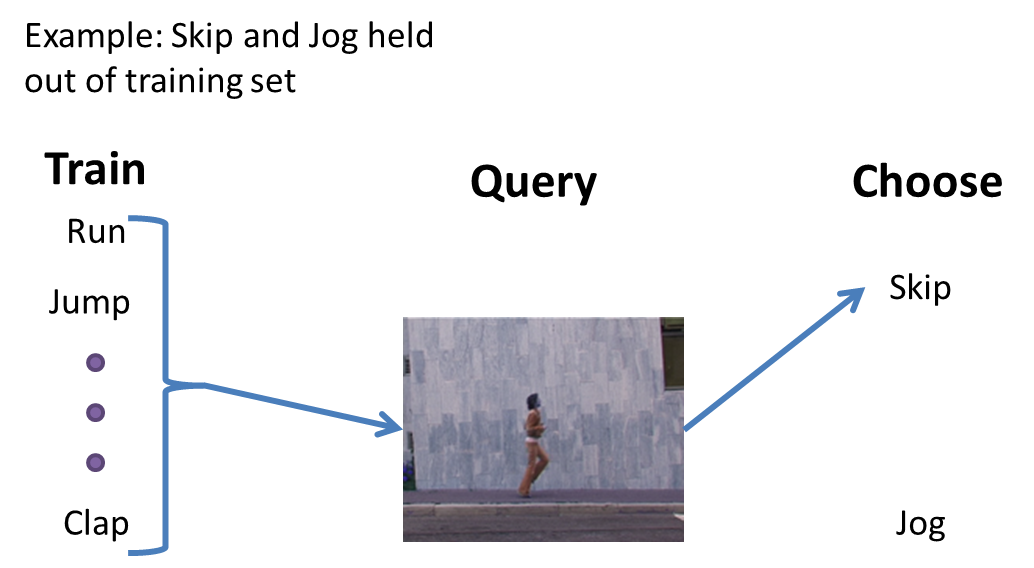
\includegraphics[width = .4\linewidth]{ltocv}
\caption{A diagram summarizing the leave-two-out cross-validation used to test zero-shot-learning.}
\label{ltocv}
\end{figure}
\subsection{Statistical Significance}
Each action has a set of 10 or more videos associated with it. With each of these videos used as a query point, we can average the success rate and assign a score for each action. The set of action scores can be compared to chance with a paired t-test to establish significance.

Chance performance at this time is estimated at 50\% correct response.  The measure we shall adopt in the final version is to establish chance with a Monte Carlo simulation of the data set. We will sever the connection between the videos and their semantic feature labels and shuffle the data. Performance of our two-stage algorithm on this shuffled set will establish a new chance baseline. Ideally this will be close to 50\%, but it may not be due to imperfections/biases in the semantic feature model.
\label{stats}
\subsection{Feature Comparison and Selection}
To see which semantic features yield the biggest advantage in decoding the action, we can test the LTOCV performance using only one semantic feature in the intermediate set. This will tells us something about what differentiates different actions effectively.

We can use the knowledge that some features perform better than others to improve overall LTOCV performance.  The best way to conduct this (so as to avoid double dipping the data set), is to feature select over the training fold of the cross-validation, and then use those selected values to evaluate the held out two actions. This will allow us to see if the features that do not do well alone somehow combine to yield good performance, or if they are noise that the classification system has difficulty ignoring.
\label{fcomp}
\subsection{Time Dependency}
Different semantic features could be more or less decodable at different points in the video examples. An interesting question one could pose is: what is the minimum length of video time needed before we can decode actions with ZSL? Additionally, which features require more or less video time before they can be reliably decoded? In general, for most applications, the less video time needed for the decoder, the better.  The semantic feature-level analysis of this phenomenon can help to further refine the semantic model.

To answer these questions, we will run our previous experiments with progressively larger action segments from the original videos, and track performance.
\label{time}
\subsection{Materials}
\subsubsection{Data Sets}
Data was taken from the following two data sets: KTH, (http://www.nada.kth.se/cvap/actions/) and Weizmann (http://www.wisdom.weizmann.ac.il/\texttildelow
vision/SpaceTimeActions.html)
\subsubsection{Semantic Features}
\label{sf}
The following are the semantic features that we selected, with values and explanations:
\begin{enumerate}
\item
$Coord\_arms$: (Discrete 0-2) 0 is no coordination, 1 is coordination, 2 is anti-coordination.
\item
$Coord\_legs$: (Discrete 0-2) 0 is none, 1 is coordination, 2 is anti-coordination.
\item
$Torso$: (Binary) 1 if torso is moving relative to the rest of the body.
\item
$Orient\_torso$: : (Discrete 0-2) 0 is that torso orientation is unrelated to the motion, 1 is that the torso is canonically parallel to motion, 2 is that the torso is canonically perpendicular to motion.
\item
$Vert$: (Discrete 0-5) amount of vertical displacement of the center of mass.
\item
$Horiz$: (Binary) 1 if there is whole body horizontal displacement.
\item
$Hand$: (Binary) 1 if the hand is lower than the center of mass, 0 if it is higher.
\item
$Speed$: (Discrete 0-5) speed of center of mass.
\item
$Limbs$: (4 features, each Discrete 1-5) speed of each of the four limbs.
\end{enumerate}
\subsubsection{Coding Libraries}
This project was coded using Python. Basic libraries used include, SciPy \cite{scipy}, NumPy \cite{numpy}, OpenCV \cite{opencv}, and The Python Image Library \cite{pil}. Ridge regression and cross-validation code taken from Scikit-learn \cite{scikit}.
\section{Preliminary Results} %Will later be Results
Oh Em Gee you guysssss

\section{Future Work} %Will later be Conclusion
At the time of submission, we estimated chance-performance as 50\% correct selections in LTOCV.  However, this may by an under-estimation of chance performance. A more rigorous way to establish statistical significance of LTOCV results is to run a Monte Carlo simulation of the entire process, as described in section \ref{stats}. This will establish a baseline to which the actual ZSL performance can be compared.
The next experiment that we plan to run is an exploration of which semantic features are the most informative for classifying the videos, by evaluating the performance of classification using each feature alone, as described in section \ref{fcomp}. This kind of experiment allows us to see where our canonical model of human actions is strongest and weakest.
Lastly, we plan to do an analysis of how much of the video is necessary for ZSL to succeed. We will run the LTOCV analysis process using progressively larger time segments of the action content sections of the videos to find the minimum amount of time needed. Furthermore, we can look at how the individual features operate on these time scales as well. The full plan is described in section \ref{time}.
\bibliographystyle{ieeetr}
\bibliography{sources}

\end{document}
